\documentclass[11pt]{exam}
\usepackage[margin=1in]{geometry}
\usepackage{amsfonts, amsmath, amssymb, amsthm}
\usepackage{mathtools}
\usepackage{enumerate}
\usepackage{listings}
\usepackage{colortbl}
\usepackage{float}
\usepackage[colorlinks,linkcolor=blue]{hyperref}

% in order to compile this file you need to get 'header.tex' from
% Canvas and change the line below to the appropriate file path
%%% theorems

\theoremstyle{plain}            % following are "theorem" style
\newtheorem{theorem}{Theorem}[section]
\newtheorem{lemma}[theorem]{Lemma}
\newtheorem{corollary}[theorem]{Corollary}
\newtheorem{proposition}[theorem]{Proposition}
\newtheorem{claim}[theorem]{Claim}
\newtheorem{fact}[theorem]{Fact}
\newtheorem{openproblem}[theorem]{Open Problem}

\theoremstyle{definition}       % following are def style
\newtheorem{definition}[theorem]{Definition}
\newtheorem{conjecture}[theorem]{Conjecture}
\newtheorem{example}[theorem]{Example}
\newtheorem{protocol}[theorem]{Protocol}
\newtheorem{exercise}[theorem]{Exercise}

\theoremstyle{remark}           % following are remark style
\newtheorem{remark}[theorem]{Remark}
\newtheorem{note}[theorem]{Note}
%\newtheorem*{solution}{Solution}

%%% special sets
\newcommand{\bit}{\ensuremath{\{0,1\}}}
\newcommand{\bitt}{\ensuremath{\{-1,1\}}}
\newcommand{\ball}{\ensuremath{\mathcal{B}}}
\newcommand{\sph}{\ensuremath{\mathbb{S}}}
\newcommand{\odisc}[2]{\ensuremath{D(#1, #2)}}
\newcommand{\cdisc}[2]{\ensuremath{\bar{D}(#1, #2)}}
\newcommand{\emp}{\varnothing}

% constants
\newcommand{\E}{\ensuremath{\mathrm{e}}}
\newcommand{\I}{\ensuremath{\mathrm{i}}}
\newcommand{\Id}{\ensuremath{\mathrm{I}}}
\newcommand{\paulix}{\ensuremath{\mathrm{X}}}
\newcommand{\pauliy}{\ensuremath{\mathrm{Y}}}
\newcommand{\pauliz}{\ensuremath{\mathrm{Z}}}

% font for general-purpose algorithms
\newcommand{\algo}[1]{\ensuremath{\mathsf{#1}}}
% font for general-purpose computational problems
\newcommand{\problem}[1]{\ensuremath{\mathsf{#1}}}
% font for complexity classes
\newcommand{\class}[1]{\ensuremath{\mathsf{#1}}}

% asymptotics
\DeclareMathOperator{\poly}{poly}
\DeclareMathOperator{\polylog}{polylog}
\DeclareMathOperator{\negl}{negl}
\DeclareMathOperator{\bigO}{O}
\DeclareMathOperator{\litO}{o}
\DeclareMathOperator{\Otil}{\tilde{O}}
\DeclareMathOperator{\Ostar}{O^*}

%%% "LEFT-RIGHT" PAIRS OF SYMBOLS

% inner product
\DeclarePairedDelimiter\inner{\langle}{\rangle}
% absolute value
\DeclarePairedDelimiter\abs{\lvert}{\rvert}
% a set
\DeclarePairedDelimiter\set{\{}{\}}
% parens
\DeclarePairedDelimiter\parens{(}{)}
% tuple, alias for parens
\DeclarePairedDelimiter\tuple{(}{)}
% square brackets
\DeclarePairedDelimiter\bracks{[}{]}
% rounding off
\DeclarePairedDelimiter\round{\lfloor}{\rceil}
% floor function
\DeclarePairedDelimiter\floor{\lfloor}{\rfloor}
% ceiling function
\DeclarePairedDelimiter\ceil{\lceil}{\rceil}
% length of some vector, element
\DeclarePairedDelimiter\length{\lVert}{\rVert}
% "lifting" of a residue class
\DeclarePairedDelimiter\lift{\llbracket}{\rrbracket}
\DeclarePairedDelimiter\len{\lvert}{\rvert}
% bra-kets
\DeclarePairedDelimiter\bra{\langle}{\rvert}
\DeclarePairedDelimiter\ket{\lvert}{\rangle}
\newcommand{\braket}[2]{\ensuremath{\langle #1 \vert #2 \rangle}}
\newcommand{\ketbra}[2]{\ensuremath{\lvert #1 \rangle \langle #2 \rvert}}

%%% spacing

\newcommand{\ws}{\hspace{1pt}}
\newcommand{\wws}{\hspace{2pt}}
\newcommand{\hs}{\hspace{4pt}}
\newcommand{\hhs}{\hspace{8pt}}
\newcommand{\hhhs}{\hspace{12pt}}

%%% LISTS

\newcommand{\oneto}{1, \ldots,}
\newcommand{\onetop}{1 \cdots,}
\newcommand{\zeroto}{0, \ldots,}
\newcommand{\zerotop}{0 \cdots,}
\newcommand{\perm}[1]{\mathbf{(#1)}}
\newcommand{\permv}[1]{(#1)}
\newcommand{\varind}[2]{#1_1, \ldots, #1_#2}
\newcommand{\varindz}[2]{#1_0, \ldots, #1_#2}
\newcommand{\varindp}[2]{#1_1 \cdots #1_#2}
\newcommand{\varindpz}[2]{#1_0 \cdots #1_#2}
\newcommand{\seq}[2]{(#1_#2)_{#2=1}^\infty}
\newcommand{\seqz}[2]{(#1_#2)_{#2=0}^\infty}

%%% MATH OPERATORS

%\DeclareMathOperator{\pr}{\mathbf{P}}
%\DeclareMathOperator{\ex}{\mathbf{E}}
\DeclareMathOperator{\pr}{P}
\DeclareMathOperator{\ex}{E}
\DeclareMathOperator{\Span}{Span}
\DeclareMathOperator{\tr}{Tr}
\DeclareMathOperator{\supp}{Supp}
\DeclareMathOperator{\im}{Im}
\DeclareMathOperator{\var}{var}
\DeclareMathOperator{\vol}{vol}
\DeclareMathOperator{\sign}{sign}
\DeclareMathOperator{\dkl}{D_{KL}}
\DeclareMathOperator{\entr}{H}
\DeclareMathOperator{\fid}{F}
\DeclareMathOperator{\dist}{D}
\DeclareMathOperator{\ad}{ad}

% hats

\newcommand{\fhat}{\ensuremath{\hat{f}}}
\newcommand{\phat}{\ensuremath{\hat{p}}}
\newcommand{\that}{\ensuremath{\hat{t}}}

%%% BLACKBOARD SYMBOLS

% \newcommand{\C}{\ensuremath{\mathbb{C}}}
\newcommand{\D}{\ensuremath{\mathbb{D}}}
\newcommand{\F}{\ensuremath{\mathbb{F}}}
% \newcommand{\G}{\ensuremath{\mathbb{G}}}
\newcommand{\J}{\ensuremath{\mathbb{J}}}
\newcommand{\N}{\ensuremath{\mathbb{N}}}
\newcommand{\Q}{\ensuremath{\mathbb{Q}}}
\newcommand{\R}{\ensuremath{\mathbb{R}}}
\newcommand{\T}{\ensuremath{\mathbb{T}}}
\newcommand{\Z}{\ensuremath{\mathbb{Z}}}
\newcommand{\QR}{\ensuremath{\mathbb{QR}}}

% sets in calligraphic type

\newcommand{\calD}{\ensuremath{\mathcal{D}}}
\newcommand{\calF}{\ensuremath{\mathcal{F}}}
\newcommand{\calG}{\ensuremath{\mathcal{G}}}
\newcommand{\calH}{\ensuremath{\mathcal{H}}}
\newcommand{\calI}{\ensuremath{\mathcal{I}}}
\newcommand{\calL}{\ensuremath{\mathcal{L}}}
\newcommand{\calN}{\ensuremath{\mathcal{N}}}
\newcommand{\calP}{\ensuremath{\mathcal{P}}}
\newcommand{\calS}{\ensuremath{\mathcal{S}}}
\newcommand{\calX}{\ensuremath{\mathcal{X}}}
\newcommand{\calY}{\ensuremath{\mathcal{Y}}}

% matrices and vectors

\newcommand{\matA}{\ensuremath{\mathbf{A}}}
\newcommand{\matB}{\ensuremath{\mathbf{B}}}
\newcommand{\matC}{\ensuremath{\mathbf{C}}}
\newcommand{\matD}{\ensuremath{\mathbf{D}}}
\newcommand{\matE}{\ensuremath{\mathbf{E}}}
\newcommand{\matF}{\ensuremath{\mathbf{F}}}
\newcommand{\matG}{\ensuremath{\mathbf{G}}}
\newcommand{\matH}{\ensuremath{\mathbf{H}}}
\newcommand{\matI}{\ensuremath{\mathbf{I}}}
\newcommand{\matJ}{\ensuremath{\mathbf{J}}}
\newcommand{\matK}{\ensuremath{\mathbf{K}}}
\newcommand{\matL}{\ensuremath{\mathbf{L}}}
\newcommand{\matM}{\ensuremath{\mathbf{M}}}
\newcommand{\matN}{\ensuremath{\mathbf{N}}}
\newcommand{\matO}{\ensuremath{\mathbf{O}}}
\newcommand{\matP}{\ensuremath{\mathbf{P}}}
\newcommand{\matQ}{\ensuremath{\mathbf{Q}}}
\newcommand{\matR}{\ensuremath{\mathbf{R}}}
\newcommand{\matS}{\ensuremath{\mathbf{S}}}
\newcommand{\matT}{\ensuremath{\mathbf{T}}}
\newcommand{\matU}{\ensuremath{\mathbf{U}}}
\newcommand{\matV}{\ensuremath{\mathbf{V}}}
\newcommand{\matW}{\ensuremath{\mathbf{W}}}
\newcommand{\matX}{\ensuremath{\mathbf{X}}}
\newcommand{\matY}{\ensuremath{\mathbf{Y}}}
\newcommand{\matZ}{\ensuremath{\mathbf{Z}}}
\newcommand{\matzero}{\ensuremath{\mathbf{0}}}

\newcommand{\veca}{\ensuremath{\mathbf{a}}}
\newcommand{\vecb}{\ensuremath{\mathbf{b}}}
\newcommand{\vecc}{\ensuremath{\mathbf{c}}}
\newcommand{\vecd}{\ensuremath{\mathbf{d}}}
\newcommand{\vece}{\ensuremath{\mathbf{e}}}
\newcommand{\vecf}{\ensuremath{\mathbf{f}}}
\newcommand{\vecg}{\ensuremath{\mathbf{g}}}
\newcommand{\vech}{\ensuremath{\mathbf{h}}}
\newcommand{\veck}{\ensuremath{\mathbf{k}}}
\newcommand{\vecm}{\ensuremath{\mathbf{m}}}
\newcommand{\vecp}{\ensuremath{\mathbf{p}}}
\newcommand{\vecq}{\ensuremath{\mathbf{q}}}
\newcommand{\vecr}{\ensuremath{\mathbf{r}}}
\newcommand{\vecs}{\ensuremath{\mathbf{s}}}
\newcommand{\vect}{\ensuremath{\mathbf{t}}}
\newcommand{\vecu}{\ensuremath{\mathbf{u}}}
\newcommand{\vecv}{\ensuremath{\mathbf{v}}}
\newcommand{\vecw}{\ensuremath{\mathbf{w}}}
\newcommand{\vecx}{\ensuremath{\mathbf{x}}}
\newcommand{\vecy}{\ensuremath{\mathbf{y}}}
\newcommand{\vecz}{\ensuremath{\mathbf{z}}}
\newcommand{\veczero}{\ensuremath{\mathbf{0}}}
\newcommand{\vecone}{\ensuremath{\mathbf{1}}}

\newcommand{\vecell}{\ensuremath{\boldsymbol\ell}}
\newcommand{\vecalpha}{\ensuremath{\boldsymbol\alpha}}
\newcommand{\vecbeta}{\ensuremath{\boldsymbol\beta}}
\newcommand{\veceta}{\ensuremath{\boldsymbol\eta}}
\newcommand{\vecmu}{\ensuremath{\boldsymbol\mu}}
\newcommand{\vecphi}{\ensuremath{\boldsymbol\phi}}
\newcommand{\vecsigma}{\ensuremath{\boldsymbol\sigma}}
\newcommand{\vectheta}{\ensuremath{\boldsymbol\theta}}
\newcommand{\vecxi}{\ensuremath{\boldsymbol\xi}}

%%% misc

\newcommand{\ind}{\ensuremath{\mathbf{1}}}

\newcommand{\congmod}[3]{#1 \equiv #2 \textrm{ modulo } #3}

\newcommand{\dee}{\,\mathrm{d}}
\newcommand{\de}{\mathrm{d}}
\newcommand{\dx}{\,\mathrm{d} x}

\newcommand{\ol}{\overline}
\newcommand{\inv}[1]{\ensuremath{#1^{-1}}}
\newcommand{\tsp}[1]{\ensuremath{#1^{\top}}}


\newcommand{\eps}{\varepsilon}
\newcommand{\ph}{\varphi}

\newcommand{\Ra}{\Rightarrow}
\newcommand{\Lra}{\Leftrightarrow}
\newcommand{\rsqa}{\rightsquigarrow}

\newcommand{\trl}{\triangleleft}
\newcommand{\trr}{\triangleright}

\newcommand{\func}[3]{#1: #2 \to #3}
\newcommand{\dd}[1]{\frac{\mathrm{d}}{\mathrm{d}#1}}
\newcommand{\ptl}[1]{\frac{\partial}{\partial #1}}
\newcommand{\prtl}[2]{\frac{\partial #1}{\partial #2}}

\newcommand{\matrixtt}[4]{
  \begin{pmatrix*}[r]
        #1 & #2 \\
        #3 & #4
    \end{pmatrix*}
}

%%% for homework and section notes

\newcommand{\commonheader}[2]{
    \pagestyle{headandfoot}
    \setlength{\headheight}{26pt}
    \setlength{\headsep}{30pt}

    \header
        {\small{\textbf{VE281: Data Structures and Algorithms}} \\ \footnotesize{\textbf{UM-SJTU Joint Institute, FA2022}}}
        {#1}
        {#2}

    \firstpageheadrule
    \runningheadrule

    \footer
        {}
        {\thepage}
        {}
}

\newcommand{\hwheader}{
    \commonheader
        {\textbf{Homework \hwnum}}
        {\small \textbf{Due at \duedate}}
}

\newcommand{\hwslnheader}{
    \commonheader
    	{}
        {\textbf{Solutions to Homework \hwnum}}
    \printanswers
}

\newcommand{\notesheader}{
    \commonheader
        {\Large \textbf{Section Notes \sectionnum}}
    	{}
}

\newcommand{\hint}[1]{
\emph{Hint}: #1
}

% for effort questions
\let\Eitem=\relax
\def\effortE{\textbf{E}~}
\makeatletter
\def\Eitem{%
    \expandafter\let\expandafter\originallabel\csname labelenum\romannumeral\@enumdepth\endcsname
    \expandafter\def\csname labelenum\romannumeral\@enumdepth\expandafter\endcsname\expandafter{%
        \expandafter\effortE\originallabel}%
    \item
    \expandafter\let\csname labelenum\romannumeral\@enumdepth\endcsname\originallabel
}
\makeatother

\allowdisplaybreaks


\geometry{left=2.5 cm,right=2.5 cm,top=2.5 cm,bottom=2.5 cm}
%\pagestyle{fancy}
\definecolor{mygreen}{rgb}{0,0.6,0}  
\definecolor{mygray}{rgb}{0.5,0.5,0.5}
\definecolor{mymauve}{rgb}{0.58,0,0.82} 
\definecolor{background}{rgb}{0.963,0.963,0.963}

\definecolor{codegreen}{rgb}{0,0.6,0}
\definecolor{codegray}{rgb}{0.5,0.5,0.5}
\definecolor{codepurple}{rgb}{0.58,0,0.82}
\definecolor{backcolour}{rgb}{0.95,0.95,0.92}

\lstdefinestyle{mystyle}{
    backgroundcolor=\color{backcolour},   
    commentstyle=\color{codegreen},
    keywordstyle=\color{magenta},
    numberstyle=\tiny\color{codegray},
    stringstyle=\color{codepurple},
    basicstyle=\ttfamily\footnotesize,
    breakatwhitespace=false,         
    breaklines=true,                 
    captionpos=b,                    
    keepspaces=true,                 
    numbers=left,                    
    numbersep=5pt,                  
    showspaces=false,                
    showstringspaces=false,
    showtabs=false,                  
    tabsize=2
}

\lstset{style=mystyle}
\newcommand{\hwnum}{3}
\newcommand{\duedate}{11:59pm, 11/27}

%\notesheader
\hwheader   % header for homework
%\hwslnheader   % header for homework solutions

% Comment the following line in order to hide solutions.
% Uncomment the line to show solutions written inside of
% LaTeX solution environments like:
%   \begin{solution}
%     My solution.
%   \end{solution}.
\printanswers

\begin{document}
\setlength{\parindent}{0pt}
\section*{Before you start:}

\subsection*{Homework Files}
You can download the starter files for coding as well as this \textit{tex} file (you only need to modify \textit{homework3.tex}) on canvas and do your homework with latex. Or you can scan your handwriting, convert to pdf file, and upload it to canvas before the due date. If you choose to write down your answers by hand, you can directly download the pdf file on canvas which provides more blank space for solution box.\\

\subsection*{Submission Form}
A pdf file as your solution named as ECE2810J\_HW3\_[Your Student ID]\_[Your name].pdf uploaded to canvas


Estimated time used for this homework: \textbf{4-5 hours.}
\\\\


\newpage
\section*{0\quad Student Info}
Your name and student id:
\begin{solution}
% Write your answer here
\end{solution}

\section{Choices (20 points)}
\subsection{Shortest distance}
Choose the shortest distance between Node 4 and Node 6.
\begin{figure}[htbp]
    \centering
    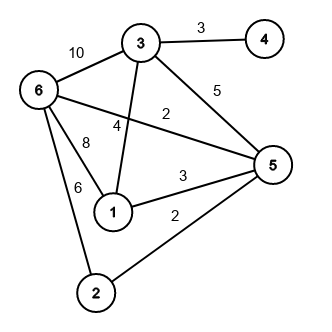
\includegraphics[height=90mm,width=90mm]{distance.png}
    \caption{Distance}
\end{figure}   
\begin{enumerate}[A)]
    \item 3
    \item 13
    \item 10
    \item 0
\end{enumerate}

\begin{solution}
    % Write your answer here
\end{solution}

\subsection{Binary indexed tree}
Binary indexed tree is like a special kind of array that can help to calculate sum from a[0] to a[n] while you can easily access or edit elements in it.
Here is one possible implement. Please choose the time complexity of $prefix\_sum$ and $add$.
\begin{lstlisting}[language=C++]
//N==1+2^a
int A[N];

int LSB (int i)
{
    return  ((i) & -(i));
}
int prefix_sum(int i) 
{
	int sum = A[0];
	for (; i != 0; i -= LSB(i))
		sum += A[i];
	return sum;
}
void add(int i, int delta) 
{
	if (i == 0) 
    {
		A[0] += delta;
		return;
	}
	for (; i < SIZE; i+= LSB(i))
		A[i] += delta;
}
\end{lstlisting}
\begin{enumerate}[A)]
    \item O(N) and O(N)
    \item O(N) and O(log N)
    \item O(log N) and O(N)
    \item O(log N) and O(log N)
\end{enumerate}

\begin{solution}
% Write your answer here
\end{solution}

\subsection{Heap}
What will the heap will be after push 20, 11. The initial heap contains : {18, 25, 32, 77, 86, 35, 93, 80}
\begin{enumerate}[A)]
    \item {18, 25, 32, 77, 86, 35, 93, 80, 20, 11}
    \item {11, 18, 20, 25, 32, 77, 86, 35, 93, 80}
    \item {11, 18, 32, 25, 20, 35, 93, 80, 77, 86} 
    \item {11, 18, 25, 32, 77, 86, 35, 93, 80, 20}
\end{enumerate}
\begin{solution}
    % Write your answer here
\end{solution}

\subsection{Spanning trees}

The number of distinct minimum spanning trees for the following weighted graph is 
\begin{figure}[htbp]
    \centering
    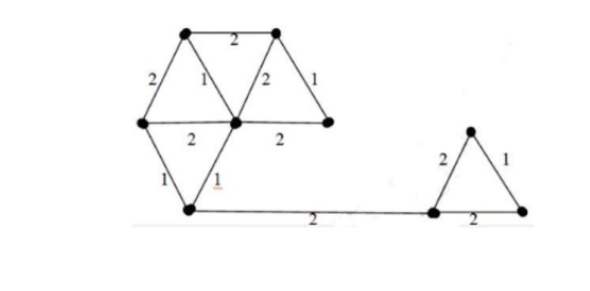
\includegraphics[height=40mm,width=90mm]{span.png}
    \caption{The weighted graph}
\end{figure}   
\begin{enumerate}[A)]
    \item 4
    \item 5
    \item 6
    \item 7
\end{enumerate}
\begin{solution}
    % Write your answer here
\end{solution}

\section{Binary Search Tree (30 points)}
\subsection{Simple simulation (16 points)}

Perform the following operations to construct a binary search tree. Show the result of the BST after each operation in either tree form or array form
(level order traversal with null pointer marked). For deletion, if it is a two-degree node, replace with the largest key in the left subtree.

\begin{enumerate}[a)]
\item Insert 21, 29, 25, 18, 19, 32, 15, 37, 22, 6, 30, 17 (3 points)
\begin{solution}
%Write your answer here.
\end{solution}

\item Delete 22 (3 points)
\begin{solution}
%Write your answer here.
\end{solution}

\item Delete 18 (3 points)
\begin{solution}
%Write your answer here.
\end{solution}

\item Insert 20 (3 points)
\begin{solution}
%Write your answer here.
\end{solution}

\item What is the in-order predecessor of node 25? What is the post-order successor of node 17? (4 points)
\begin{solution}
%Write your answer here.
\end{solution}


\end{enumerate}

\newpage
\subsection{Better than linear selection? (13 points)}
After learning the application of the BST, Jeremy thinks that with BST, rank search
can be done either in a faster way or with less space compared with the linear selection
algorithms introduced in the lecture.
\begin{enumerate}[a)]
    \item Compare BST rank search with deterministic selection algorithm in
    terms of time complexity and space usage. Assume that for each node, a variable
    $left\_size$ is maintained as introduced in the lecture. (7 points)
    \begin{solution}
    %Write your answer here.
    \\ \hspace*{\fill} \\
    \\ \hspace*{\fill} \\
    \\ \hspace*{\fill} \\
    \\ \hspace*{\fill} \\
    \\ \hspace*{\fill} \\
    \\ \hspace*{\fill} \\
    \end{solution}
    \newpage
    \item However, master of algorithm, has a different idea again. He states that for the linear selection algorithm, the input can be arbitrary array while for BST rank search, you have to first build up a binary search tree from the arbitrary array, which will also take some time. Therefore, the average time complexity of BST rank search is not better than $O(n)$. Is he right? (7 points)\\
    Assume that we are working on a fixed array and doing lots of rank search.
    \begin{solution}
    %Write your answer here.
    \\ \hspace*{\fill} \\
    \\ \hspace*{\fill} \\
    \\ \hspace*{\fill} \\
    \\ \hspace*{\fill} \\
    \\ \hspace*{\fill} \\
    \\ \hspace*{\fill} \\
    \end{solution}
\end{enumerate}

\newpage
\section{Proof Questions(30 points)}
    \subsection{Order of deletion(5 points)}
    Does the deletion of two nodes in BST exchangeable? For example, we want to delete node $x$ and $y$, if the result of first deleting $x$ then $y$ is the same with first $y$ then $x$, then it's called exchangeable. If you agree, give a brief proof. If you disagree, give a example.
    \begin{solution}
    % Write your answer here
    \\ \hspace*{\fill} \\
    \\ \hspace*{\fill} \\
    \\ \hspace*{\fill} \\
    \\ \hspace*{\fill} \\
    \\ \hspace*{\fill} \\
    \\ \hspace*{\fill} \\
    \\ \hspace*{\fill} \\
    \\ \hspace*{\fill} \\
    \\ \hspace*{\fill} \\
    \\ \hspace*{\fill} \\
    \\ \hspace*{\fill} \\
    \\ \hspace*{\fill} \\
    \\ \hspace*{\fill} \\
    \\ \hspace*{\fill} \\
    \\ \hspace*{\fill} \\
    \\ \hspace*{\fill} \\
    \\ \hspace*{\fill} \\
    \\ \hspace*{\fill} \\
    \end{solution}
     
    \newpage
    \subsection{Transverse of a tree(10 points)}
    In the three orders of transverse taught in class, we will use the recursion to do the transverse. And can you give a way of transverse without using recursion? And also show what kind of transverse it is. (One simple way is to use the idea of topological sort taught in class, and you can also try to think how to do all the three tranverses, but it's not required)\par \par 
    \begin{solution}
    % Write your answer here
    \\ \hspace*{\fill} \\
    \\ \hspace*{\fill} \\
    \\ \hspace*{\fill} \\
    \\ \hspace*{\fill} \\
    \\ \hspace*{\fill} \\
    \\ \hspace*{\fill} \\
    \\ \hspace*{\fill} \\
    \\ \hspace*{\fill} \\
    \\ \hspace*{\fill} \\
    \\ \hspace*{\fill} \\
    \\ \hspace*{\fill} \\
    \\ \hspace*{\fill} \\
    \\ \hspace*{\fill} \\
    \\ \hspace*{\fill} \\
    \\ \hspace*{\fill} \\
    \\ \hspace*{\fill} \\
    \\ \hspace*{\fill} \\
    \\ \hspace*{\fill} \\
    \end{solution}

\section{Appliaction(20 points)}
    \subsection{New Edge in BST(5 points)}
    Suppose we now have a tree. Try to prove that, if a new edge is added, there should be a cycle.\par 
    \begin{solution}
    % Write your answer here
    \\ \hspace*{\fill} \\
    \\ \hspace*{\fill} \\
    \\ \hspace*{\fill} \\
    \\ \hspace*{\fill} \\
    \\ \hspace*{\fill} \\
    \\ \hspace*{\fill} \\
    \\ \hspace*{\fill} \\
    \\ \hspace*{\fill} \\
    \\ \hspace*{\fill} \\
    \\ \hspace*{\fill} \\
    \\ \hspace*{\fill} \\
    \\ \hspace*{\fill} \\
    \end{solution}
    \newpage
    \subsection{New Edge in MST(5 points)}
    Suppose edge $(u,v)$ is one edge in a connected graph with the minimum weight. Prove that this edge is in at least one minimum span tree of the graph.\par 
    \begin{solution}
    % Write your answer here
    \\ \hspace*{\fill} \\
    \\ \hspace*{\fill} \\
    \\ \hspace*{\fill} \\
    \\ \hspace*{\fill} \\
    \\ \hspace*{\fill} \\
    \\ \hspace*{\fill} \\
    \\ \hspace*{\fill} \\
    \\ \hspace*{\fill} \\
    \\ \hspace*{\fill} \\
    \\ \hspace*{\fill} \\
    \\ \hspace*{\fill} \\
    \\ \hspace*{\fill} \\
    \end{solution}
    \newpage
    \subsection{K's smallest number(10 points)}
    Suppose we have a binary search tree. Output the k's smallest number of the tree. Write the pseudocode or C++ code under. You can just call the root of the tree $root$\par 
    The difinition of the node and function in C++ is shown below:
    \begin{lstlisting}[language = C++]
    Struct TreeNode{
       int data;
       TreeNode* left, right; 
    }
    int kthSmallest(TreeNode* root, int k)
    \end{lstlisting}
    Write your answer here.
    \clearpage
    
\newpage
\section{Coding question for you to practice}
This part will not be counted for you homework score, just for you to practice.
\begin{enumerate}
    \item Leetcode 207 course-schedule
    \item Leetcode 114 flatten-binary-tree-to-linked-list
    \item Leetcode 100 same-tree
    \item Leetcode 130 surrounded-regions
    \item Leetcode 102 binary-tree-level-order-traversal
    \item Leetcode 127 word-ladder
    \item Leetcode 208 implement-trie-prefix-tree
    \item Leetcode 218 the-skyline-problem
    \item Leetcode 18  4sum
    \item Leetcode 264 ugly-number-ii
\end{enumerate}
\end{document}